%!TEX options=--shell-escape
\documentclass[tikz]{standalone}
\usepackage[T1]{fontenc}
\usepackage[utf8]{inputenc}
\usepackage{xcolor}
\usepackage{amsmath}
\usepackage{amssymb}
\usepackage{hyperref}
\usepackage{accsupp}    
\usepackage{graphicx}
\usepackage{mathtools}
\usepackage{pagecolor}
\usepackage{amsmath} % for \dfrac
\usepackage{tikz}
\tikzset{>=latex} % for LaTeX arrow head
\usepackage{pgfplots} 
\usepackage[edges]{forest}
\usetikzlibrary{patterns, backgrounds, arrows.meta}
\setlength{\parindent}{0cm}
\setlength{\parskip}{1em}
\usepackage{braket}

\usetikzlibrary{patterns}
\def\rescale{0.142857}

\begin{document}
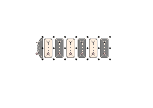
\begin{tikzpicture}[scale=\rescale]

   \foreach \x in {0, 2,...,4}{
        \fill[line width = 0.25 * \rescale, draw=black, fill=yellow!40!red!10, rounded corners = \rescale * 3pt] (\x + 0.15, 0.15) rectangle (\x+0.85, 1.85) ;
        \fill[line width = 0.25 * \rescale, draw=black, fill=gray, rounded corners = \rescale * 3pt] (\x + 1.15, 0.15) rectangle (\x+1.85, 1.85) ;
    }

   \fill[line width = 0.25 * \rescale, draw=black, fill=gray, rounded corners=\rescale * 5pt] (0, 0) to [bend left=45](0, 2) -- cycle ;

    \foreach \x in {0, 2,...,4}{
           \draw[line width = \rescale,  dash pattern={on 0.5pt off 0.5pt on 0.5pt off 0.5pt}, yellow!40!red!10] (\x+1, 0) -- (\x+1.5, 0.5);
           \draw[line width = \rescale,  dash pattern={on 0.5pt off 0.5pt on 0.5pt off 0.5pt}, yellow!40!red!10] (\x+2, 0) -- (\x+1.5, 0.5);
           \draw[line width = \rescale,  dash pattern={on 0.5pt off 0.5pt on 0.5pt off 0.5pt}, yellow!40!red!10] (\x+1, 2) -- (\x+1.5, 1.5);
           \draw[line width = \rescale,  dash pattern={on 0.5pt off 0.5pt on 0.5pt off 0.5pt}, yellow!40!red!10] (\x+2, 2) -- (\x+1.5, 1.5);
           \draw[line width = \rescale,  dash pattern={on 0.5pt off 0.5pt on 0.5pt off 0.5pt}, yellow!40!red!10] (\x+1.5,0.5) -- (\x+1.5, 1.5);

           \draw[line width = \rescale,  dash pattern={on 0.5pt off 0.5pt on 0.5pt off 0.5pt}, gray] (\x, 0) -- (\x+0.5, 0.5);
           \draw[line width = \rescale,  dash pattern={on 0.5pt off 0.5pt on 0.5pt off 0.5pt}, gray] (\x+1, 0) -- (\x+0.5, 0.5);
           \draw[line width = \rescale,  dash pattern={on 0.5pt off 0.5pt on 0.5pt off 0.5pt}, gray] (\x, 2) -- (\x+0.5, 1.5);
           \draw[line width = \rescale,  dash pattern={on 0.5pt off 0.5pt on 0.5pt off 0.5pt}, gray] (\x+1, 2) -- (\x+0.5, 1.5);
           \draw[line width = \rescale,  dash pattern={on 0.5pt off 0.5pt on 0.5pt off 0.5pt}, gray] (\x+0.5,0.5) -- (\x+0.5, 1.5);


    }
    \draw[line width = \rescale,  dash pattern={on 0.5pt off 0.5pt on 0.5pt off 0.5pt}, yellow!40!red!10] (0, 0) to [bend left=-45](-0.5, 0.5);
    \draw[line width = \rescale,  dash pattern={on 0.5pt off 0.5pt on 0.5pt off 0.5pt}, yellow!40!red!10] (0, 2) to [bend left=45](-0.5, 1.5);
    \draw[line width = \rescale,  dash pattern={on 0.5pt off 0.5pt on 0.5pt off 0.5pt}, yellow!40!red!10] (-0.5, 1.5) to [bend left=45](-0.5, 0.5);



    \foreach \x in {0, 1, ...,6}{
           \filldraw[line width = 0.25 * \rescale, draw=black, fill=black] (\x, 0) circle[radius=2pt] node[font=\tiny] {};
           \filldraw[line width = 0.25 * \rescale, draw=black, fill=black] (\x, 1) circle[radius=2pt] node[font=\tiny] {};
           \filldraw[line width = 0.25 * \rescale, draw=black, fill=pink!60] (\x - 0.5, 0.5) circle[radius=3pt] node[font=\tiny] {};

           \filldraw[line width = 0.25 * \rescale, draw=black, fill=black] (\x, 2) circle[radius=2pt] node[font=\tiny] {};
           \filldraw[line width = 0.25 * \rescale, draw=black, fill=pink!60] (\x - 0.5, 1.5) circle[radius=1pt] node[font=\tiny] {};
           \filldraw[opacity=0, line width = 0.25 * \rescale, draw=black, fill=black] (\x, -1) circle[radius=2pt] node[font=\tiny] {};

    }

    \filldraw[line width = 0.25 * \rescale, draw=black, fill=pink!60, opacity=0] (6.5, 0.5) circle[radius=3pt] node[font=\tiny] {};


\end{tikzpicture} 
\end{document}

